\documentclass[12pt]{article}
\usepackage{amsmath,amsthm,booktabs,subfigure,anysize,hyperref,graphicx,float,bbm,epstopdf}
\usepackage[margin=1in]{geometry}
\bibliographystyle{aea}

\usepackage{threeparttable}
\usepackage{array}
\usepackage{booktabs}
\usepackage{multirow}
\usepackage{xcolor}
\usepackage{bm}
\definecolor{dark-red}{rgb}{0.4,0.15,0.15}
\definecolor{dark-blue}{rgb}{0.15,0.15,0.4}
\definecolor{medium-blue}{rgb}{0,0,0.5}
\definecolor{ChadBlue}{rgb}{.1,.1,.5}
\definecolor{ChadDarkBlue}{rgb}{.1,0,.1}
\definecolor{ChadBlue}{rgb}{.1,.1,.5}
\definecolor{ChadRoyal}{rgb}{.2,.2,.8}
\definecolor{ChadGreen}{rgb}{0,.4,0}
\definecolor{ChadRed}{rgb}{.5,0,.5}
\hypersetup{
    colorlinks, linkcolor=ChadRed,
    citecolor=ChadBlue, urlcolor=ChadBlue
}
\newcommand\posscite[1]{\citeauthor{#1}'s (\citeyear{#1})}
\setlength{\parskip}{0.15cm}
\newtheorem{proposition}{\color{ChadGreen} Proposition}
\newtheorem{finding}{\color{ChadGreen} Finding}
\newtheorem{SF}{\color{ChadGreen} Stylized fact}
\newtheorem{hyp}{Hypothesis}
\newtheorem{fact}{Fact}
\newtheorem{prop}{Proposition}
\usepackage{caption}
\usepackage[font=small,labelfont=bf]{caption}
\usepackage{amssymb}
\usepackage{amsfonts}
\usepackage{amsmath}
\usepackage{accents}
\usepackage{color,soul}
\usepackage{smartdiagram}
\usepackage[figuresright]{rotating} % Rotating table
\usepackage{lscape} % Rotating table
\usepackage{diagbox}
\usepackage{multicol}
\usepackage{tikz}
\usepackage{comment}
\usepackage{float}
\usepackage{natbib}

\newcommand{\ubar}[1]{\underaccent{\bar}{#1}}
\usepackage[all]{hypcap}

\newtheorem{theorem}{Theorem}
\newtheorem{cor}[theorem]{Corollary}
\renewcommand{\proof}{\noindent \textbf{Proof.\ }}
\newtheorem{conjecture}{Conjecture}
\newtheorem{example}{Example}
\newtheorem{defn}{Definition}
\renewcommand{\qed}{\hfill\rule{2.1mm}{2.1mm}}
\newcommand\fnote[1]{\captionsetup{font=small}\caption*{#1}}

\let\LaTeXtitle\title
\renewcommand{\arraystretch}{1.1} % space between rows
\usepackage{sectsty}
\usepackage{lscape}
\graphicspath{{figure/}}
\newcolumntype{P}[1]{>{\centering\arraybackslash}p{#1}}

\linespread{1.2}
\geometry{a4paper,scale=0.75}
\setlength{\parskip}{0.5em}


%---------------------------------------------------------------------------------------

\begin{document}

\title{\Large \textbf{Global Monetary Policy Shocks and Export Prices}}


\author{\large \href{http://yaoli.people.ust.hk/}{Yao Amber Li}\thanks{Li: Department of Economics and Faculty Associate of the Institute for Emerging Market Studies (IEMS), The Hong Kong University of Science and Technology, Hong Kong}\\ \large{HKUST}
\medskip
\and \href{}{Lingfei Lu}\thanks{Lu: Department of Economics, The Hong Kong University of Science and Technology, Hong Kong } \\ \large{HKUST}
\medskip
\and \href{}{Jingbo Yao}\thanks{Yao: Department of Economics, The Hong Kong University of Science and Technology, Hong Kong} \\ \large{HKUST}
}
\date{\today}

\maketitle

\tableofcontents
\newpage

\section{Introduction}



\subsection{Background and motivation}

How export price responds to international shocks is essential in international economics. People usually focus on exchange rate shocks, productivity shocks, and other real demand and cost shocks; less attention is drawn to international monetary policy shocks. Tons of literature have revealed the domestic and spillover effects of monetary policy shocks on the real economy and asset prices, but few people study their implications on the pricing behavior of export firms. It is found that export firms even suffer more from the global financial cycle than domestic firms. In an era of growing global financial and trade integration, the significance of addressing this question becomes even more pronounced, which may deepen our understanding of the international transmission of monetary shocks and the interaction between trade and the financial market.

This is the first paper to investigate how international monetary policy shocks affect export prices with detailed firm-product level data. 

\subsection{This paper}

China is the biggest export country in the world, and using China as an example has general implications. By integrating Chinese custom data with CIE data, our investigation reveals substantial heterogeneity in the responses of firm export prices to international monetary policy shocks, gauged through high-frequency asset price fluctuations. In particular, our analysis delves into the influence of major global central banks, uncovering noteworthy patterns. Notably, a tightening monetary policy shock in the United States substantially elevates China's export prices, whereas European stocks exert a contrasting effect by diminishing export prices. Conversely, shocks emanating from the United Kingdom and Japan exhibit negligible impacts.

The pattern of European shock is consistent with the demand shrink effect. However, as the main driver of the global financial cycle, the US monetary shock also exerts a supple-side effect on China's export prices and dominates the demand-side impact. More specifically, we reveal that tightening US monetary policy worsens the credit conditions of China's exporting firms by raising the borrowing cost and reducing the liquid assets, which drives the rise of export prices. 

\subsection{Literature and contribution}

This paper contributes to three strands of literature:


\begin{enumerate}

\item Determinants of firm pricing behaviors

Exchange rate pass-through papers study how export prices respond to exchange rate shocks, like \cite{obstfeld2000six}, \cite{amiti2014importers}, \cite{li2015exchange}, \cite{devereux2017importers}, \cite{auer2018quality}. Also, some papers investigate the impact of firm characteristics, destinations, and trade liberalization on export prices (e.g. \cite{manova2012export}, \cite{fan2015credit}, \cite{harrigan2015export}, \cite{fan2015trade}, etc.). Compared with these papers, we analyze the impact of international monetary policy shocks on export prices.

\item Global monetary policy spillover\\
Many papers investigate the spillover effect of international monetary policy shocks either on the real economy (see \cite{kim2001international}, \cite{faust2003monetary}, \cite{faust2003identifying}, \cite{mackowiak2007external}, \cite{di2008impact}, \cite{bluedorn2011open}) or on asset prices (like \cite{craine2008international}, \cite{wongswan2009response}, \cite{hausman2011global}, \cite{rogers2014evaluating}, \cite{miranda2020us}). Regarding the impact on trade, some open macroeconomic literature has implications on how monetary shock affects the current account (like \cite{obstfeld1995exchange}). Empirically, \cite{lin2018international} investigates how US monetary policy affects global trade volume using country-sector data. However, Our paper is the first paper to focus on the impact on export prices.

\item The role of financial friction in international trade.\\
Existing literature reveals how financial friction affects exports, like \cite{manova2013credit}, \cite{fan2015credit}, \cite{manova2015firm}, \cite{lin2018international}, etc. Compared with these papers, we study, given the existence of financial friction, how monetary policy affects export prices through the change of credit conditions. 

\end{enumerate}

\section{Main results}

\subsection{Benchmark regression}

\begin{equation}
    \Delta \ln P_{it} = \alpha+\beta \cdot brw_{t}+ \Gamma \cdot \textbf{Z}_{it-1}+\xi_{i}+\varepsilon_{i t}
\end{equation}


Benchmark: use firm aggregate price, monthly data
- Positive and significant, add year FE also hold

\begin{center}
\begin{tabular}{l*{4}{c}}
\toprule
            &\multicolumn{1}{c}{(1)}   &\multicolumn{1}{c}{(2)}   &\multicolumn{1}{c}{(3)}   &\multicolumn{1}{c}{(4)}   \\
\midrule
brw         &       0.187***&       0.149***&       0.042***&       0.058***\\
            &     (0.011)   &     (0.011)   &     (0.011)   &     (0.010)   \\
\addlinespace
L.dlnprice\_YoY&               &       0.302***&               &       0.300***\\
            &               &     (0.003)   &               &     (0.003)   \\
\addlinespace
Firm FE     &         Yes   &         Yes   &         Yes   &         Yes   \\
\addlinespace
Year FE     &          No   &          No   &         Yes   &         Yes   \\
\midrule
\(N\)       &     1108044   &      946438   &     1108044   &      946438   \\
\bottomrule
\multicolumn{5}{l}{\footnotesize Standard errors in parentheses}\\
\multicolumn{5}{l}{\footnotesize * \(p<0.1\), ** \(p<0.05\), *** \(p<0.01\)}\\
\end{tabular}
\end{center}

Note: Column (1)(2): firm FE; Column (3)(4): firm FE and year FE. All clusters are at the firm level.

\textcolor{blue}{TBD: Need to add control like firm size, firm productivity, and exchange rate change, etc.}

\subsection{Robustness}

(1) Using lag values of brw

\begin{equation}
    \Delta \ln P_{it} = \alpha + \beta \cdot \sum^{N}_{n=1}  brw_{t-n}+ \Gamma \cdot \textbf{Z}_{it-1}+\xi_{i}+\varepsilon_{i t}
\end{equation}

\begin{center}
\begin{tabular}{l*{4}{c}}
\toprule
            &\multicolumn{1}{c}{(1)}   &\multicolumn{1}{c}{(2)}   &\multicolumn{1}{c}{(3)}   &\multicolumn{1}{c}{(4)}   \\
\midrule
L.brw       &       0.166***&               &               &               \\
            &     (0.012)   &               &               &               \\
\addlinespace
brw\_lag3    &               &       0.111***&               &               \\
            &               &     (0.008)   &               &               \\
\addlinespace
brw\_lag6    &               &               &       0.131***&               \\
            &               &               &     (0.007)   &               \\
\addlinespace
brw\_lag12   &               &               &               &       0.072***\\
            &               &               &               &     (0.006)   \\
\addlinespace
Firm FE     &         Yes   &         Yes   &         Yes   &         Yes   \\
\midrule
\(N\)       &     1045563   &      949715   &      829476   &      662749   \\
\bottomrule
\multicolumn{5}{l}{\footnotesize Standard errors in parentheses}\\
\multicolumn{5}{l}{\footnotesize * \(p<0.1\), ** \(p<0.05\), *** \(p<0.01\)}\\
\end{tabular}
\end{center}

Note: Column (1), brw in the last month; Column (2), sum of brw in the last three months; Column (3), sum of brw in the last six months; Column (4), sum of brw in the last 12 months.

(2) Using firm-product level price, monthly data, no year fixed effect: \footnote{Using product level price has two shortcomings: (i) many dimensions in the dependent variables, but the explanatory variable only has one dimension, so there are many noises. To alleviate it, we can control past price levels and price changes; (ii) Sometimes, the product scope of the exporting firm may change.}



\begin{equation}
    \Delta \ln P_{hit} = \alpha+\beta \cdot brw_{t}+ \Gamma \cdot \textbf{Z}_{it-1}+\xi_{hi}+\varepsilon_{hi t}
\end{equation}

Lag effects with different time horizons are all positive and significant, but it is weaker with year FE.


\begin{tabular}{l*{6}{c}}
\toprule
            &\multicolumn{1}{c}{(1)}   &\multicolumn{1}{c}{(2)}   &\multicolumn{1}{c}{(3)}   &\multicolumn{1}{c}{(4)}   &\multicolumn{1}{c}{(5)}   &\multicolumn{1}{c}{(6)}   \\
\midrule
brw         &       0.144***&       0.118***&       0.019*  &       0.041***&       0.159***&       0.119***\\
            &     (0.011)   &     (0.011)   &     (0.011)   &     (0.011)   &     (0.014)   &     (0.014)   \\
\addlinespace
L.dlnprice\_hit\_YoY&               &       0.273***&               &       0.272***&               &       0.322***\\
            &               &     (0.002)   &               &     (0.002)   &               &     (0.005)   \\
\addlinespace
Firm-product FE&         Yes   &         Yes   &         Yes   &         Yes   &          No   &          No   \\
\addlinespace
Firm FE     &          No   &          No   &          No   &          No   &         Yes   &         Yes   \\
\addlinespace
Year FE     &          No   &          No   &         Yes   &         Yes   &          No   &          No   \\
\addlinespace
Product FE  &          No   &          No   &          No   &          No   &         Yes   &         Yes   \\
\midrule
\(N\)       &     2455577   &     1824336   &     2455577   &     1824336   &     2494529   &     1842588   \\
\bottomrule
\multicolumn{7}{l}{\footnotesize Standard errors in parentheses}\\
\multicolumn{7}{l}{\footnotesize * \(p<0.1\), ** \(p<0.05\), *** \(p<0.01\)}\\
\end{tabular}

(3) Using firm-product-country level price, annual data.

(4) Alternative measures of monetary policy shocks: Nakamura and Steinsson shock and Fed fund rate shock

\begin{center}
\begin{tabular}{l*{4}{c}}
\toprule
            &\multicolumn{1}{c}{(1)}   &\multicolumn{1}{c}{(2)}   &\multicolumn{1}{c}{(3)}   &\multicolumn{1}{c}{(4)}   \\
\midrule
NS\_shock    &       0.150***&       0.139***&               &               \\
            &     (0.009)   &     (0.009)   &               &               \\
\addlinespace
ffr\_shock   &               &               &       0.026***&       0.023***\\
            &               &               &     (0.007)   &     (0.007)   \\
\addlinespace
L.dlnprice\_YoY&               &       0.302***&               &       0.303***\\
            &               &     (0.003)   &               &     (0.003)   \\
\addlinespace
Firm FE     &         Yes   &         Yes   &         Yes   &         Yes   \\
\midrule
\(N\)       &     1108044   &      946438   &     1108044   &      946438   \\
\bottomrule
\multicolumn{5}{l}{\footnotesize Standard errors in parentheses}\\
\multicolumn{5}{l}{\footnotesize * \(p<0.1\), ** \(p<0.05\), *** \(p<0.01\)}\\
\end{tabular}
\end{center}
(5) Invoicing currency concern

One may argue that the invoicing currency matters in price elasticity. However, due to data limitation, the invoicing currency of each firm is unknown, so the price in RMB increases does not necessarily mean that the price also increases in the true invoicing currency. 

Actually, although we do not know the detailed invoicing currency for each product, most of these products are denominated in USD or RMB. Before July 2005, because of the fixed exchange rate, invoicing by RMB was equivalent to by USD, so price change in RMB and USD is similar. 

We will use both nominal prices denominated in RMB and USD.

(6) Is the average export price increase driven by some specific countries?
That is not the case because nearly all the main countries experienced price increases. Test whether certain destinations drive the price change, we use alternative subsamples with only certain countries.
 

(7) Single-product firms

Aggregate firm-product-country level prices into firm-level prices may cancel out some price changes. Also, it would be possible for an exporting firm may switch their export product mix when facing credit constraints. A more thorough analysis calls for further investigation of resource reallocation across core versus non-core product products within a firm, but this would be out of the scope of the current paper. So, we use a subsample with single-product firms.


\section{Decomposition}

In this section, we will decompose export prices into markups and marginal costs to find the reasons for price changes.

\subsection{Markup vs marginal cost}

Following \cite{}, we can estimate the firm-level markup without direct prices and marginal cost measures using the structural assumptions of \cite{dlw2012} and the GMM estimation method.

\begin{equation}
    \Delta Markup_{it} = \alpha +\beta \cdot brw_{t}+ \Gamma \cdot \textbf{Z}_{it-1}+\xi_{i}+\varepsilon_{it} 
\end{equation}

\begin{equation}
    \Delta \ln P_{it} = \alpha+\beta \cdot brw_{t}+ \gamma \cdot \Delta Markup_{it}+ \Gamma \cdot \textbf{Z}_{it-1}+\xi_{i}+\varepsilon_{i t} 
\end{equation}

Tight monetary policy shocks lead to lower firm-level markups, so marginal costs are the main driver of export price increases.


\textcolor{blue}{TBD: Divide firms into high-markup and low-markup groups. Low-markup firms may be hard to adjust their markup and they consist of the majority of Chinese exporters. In a longer period, the variable markup channel may be more important because the average markup of Chinese firms increases.} 

\begin{center}
\begin{tabular}{l*{4}{c}}
\toprule
            &\multicolumn{1}{c}{(1)}&\multicolumn{1}{c}{(2)}&\multicolumn{1}{c}{(3)}&\multicolumn{1}{c}{(4)}\\
            &\multicolumn{1}{c}{S12.Markup}&\multicolumn{1}{c}{S12.Markup}&\multicolumn{1}{c}{dlnprice\_YoY}&\multicolumn{1}{c}{dlnprice\_YoY}\\
\midrule
brw         &      -0.023***&               &       0.181***&               \\
            &     (0.008)   &               &     (0.013)   &               \\
\addlinespace
brw\_lag12   &               &      -0.057***&               &       0.073***\\
            &               &     (0.010)   &               &     (0.007)   \\
\addlinespace
S12.Markup&               &               &       0.006** &       0.010***\\
            &               &               &     (0.003)   &     (0.004)   \\
\addlinespace
Firm FE     &         Yes   &         Yes   &         Yes   &         Yes   \\
\midrule
\(N\)       &      836110   &      472282   &      773718   &      451708   \\
\bottomrule
\multicolumn{5}{l}{\footnotesize Standard errors in parentheses}\\
\multicolumn{5}{l}{\footnotesize * \(p<0.1\), ** \(p<0.05\), *** \(p<0.01\)}\\
\end{tabular}
\end{center}


\subsection{Cost decomposition}

Cross-validation cost/sales \\
unit of borrowing cost significantly positive, unit labor cost (wage) decrease
 

\section{Mechanism}

\subsection{Discussion}

The literature has confirmed that contractionary U.S. monetary policy shocks will lead to the tightening of foreign financial conditions: interest rate increases, credit shrinking, bank deleveraging, and retrenchments of international credit flows. Although the impacts vary across the receiving country's characteristics, such as trade and financial integration, financial openness, exchange rate regime, financial market development, labor market rigidities, industry structure, and participation in global value chains.  

\begin{enumerate}

\item “\textit{U.S. monetary policy shocks induce comovements in the international financial variables that characterize the “Global Financial Cycle.” A single global factor that explains an important share of the variation of risky asset prices around the world decreases significantly after a U.S. monetary tightening. Monetary contractions in the US lead to significant deleveraging of global financial intermediaries, a decline in domestic credit provision globally, strong retrenchments of international credit flows, and tightening of foreign financial conditions. Countries with floating exchange rate regimes are subject to similar financial spillovers.}” -- Miranda-Agrippino, Silvia, and Hélene Rey. "US monetary policy and the global financial cycle." The Review of Economic Studies 87.6 (2020): 2754-2776.

\item "\textit{First, several papers investigate the global output spillovers from conventional US monetary policy (see, for example, Kim, 2001; Faust and Rogers, 2003; Faust et al., 2003; Mackowiak, 2007; Di Giovanni and Shambaugh, 2008; Bluedorn and Bowdler, 2011). The results of this literature suggest that US monetary policy has substantial global spillovers across both advanced and emerging market economies and that these arise mainly through spillovers in interest rates.}" -- Georgiadis, Georgios. "Determinants of global spillovers from US monetary policy." Journal of International Money and Finance 67 (2016): 41-61.

\item “\textit{The magnitude of spillovers depends on the receiving country's trade and financial integration, financial openness, exchange rate regime, financial market development, labor market rigidities, industry structure, and participation in global value chains. The role of these country characteristics for the spillovers often differs across advanced and non-advanced economies and also involves non-linearities. The results of this paper suggest that policymakers could mitigate their economies' vulnerability to US monetary policy by fostering trade integration as well as domestic financial market development, increasing the flexibility of exchange rates, and reducing frictions in labor markets.}”-- Georgiadis, Georgios. "Determinants of global spillovers from US monetary policy." Journal of International Money and Finance 67 (2016): 41-61.

\item \cite{RePEc:fip:fedkpr:y:2013:x:9} has shown that capital flows and stock prices in most countries, regardless of their exchange rate regime against the dollar, display strong comovements with the global cycle.

\end{enumerate}


Actually, although China has capital control, Prasad and Wei (2005) report that there have been huge capital inflows into China since 2003 that cannot be explained by trade surplus or foreign direct investments. Such international capital is referred as “hot money.” Investors attempt to earn short-term profits by observing interest rate differences or through anticipated currency revaluations or expected returns from holding securities (Kim and Singal, 2000). Although China has adopted various measures to restrict volatile international short-term capital flows that are speculative in nature, speculators continue to circumvent Chinese laws and regulations. Martin and Morrison (2008) indicate that more than half of the hot money flown into China takes the form of over-reported or forged FDI. China is not fully isolated from hot money inflows because capital controls are not applied to all capital accounts transaction categories and several of these categories are loosely managed (Xie, 2004). So, we can treat China as a partially capital-free country, and the channels discussed in \cite{miranda2020us} still apply to China.

What's more, although China is found to be restrictive to portfolio flows, it is quite open to FDI inflows. \cite{lin2018foreign} reveal that there exists a trade credit channel through which FDI firms can propagate global liquidity shocks to the host economy despite its tight controls on non-FDI financial flows.

 
To sum up, no matter whether through financial intermediaries, global asset prices, or trade provisions, all the previous literature implies that US tightening may increase Chinese firms' borrowing costs and decrease their liquidity. In light of this, we provide two hypotheses:
\begin{enumerate}
    \item \textbf{Global borrowing cost channel}. Tightening US monetary shock deteriorates the financing environment and increases the borrowing cost of firms forcing them to offset this cost by lifting prices.
    \item \textbf{Global liquidity channel}. Tightening US monetary shock decreases the liquidity of export firms either through bank and trade credit shrink or through reduction of operational income, which induces firms to raise prices to alleviate liquidity constraints.
\end{enumerate}


\subsection{Regression}

\subsubsection{The impact of US shock on borrowing cost and liquidity}

$$
\Delta \ln Y_{it} = \alpha +\beta \cdot brw_{t}+X_{it}+\xi_{i}+\varepsilon_{i t}
$$

where $Y$ is the firm's borrowing cost and liquidity. To be consistent with the frequency of dependent variables, here we aggregate US shock in the year level.

Consistent with previous literature, the borrowing cost increases (see Figure \ref{fig: brw_IEoL_Cash} Columns 1-2). Liquidity ratio decreases (see Columns 3-4). The conclusion of \cite{lin2018foreign} is also verified (see Columns 5-6) that trade provision decreases after a contractionary US shock.

\begin{center}
\begin{tabular}{l*{6}{c}}
\toprule
            &\multicolumn{1}{c}{(1)}&\multicolumn{1}{c}{(2)}&\multicolumn{1}{c}{(3)}&\multicolumn{1}{c}{(4)}&\multicolumn{1}{c}{(5)}&\multicolumn{1}{c}{(6)}\\
            &\multicolumn{1}{c}{D.IEoL}&\multicolumn{1}{c}{D.IEoL}&\multicolumn{1}{c}{D.Cash}&\multicolumn{1}{c}{D.Cash}&\multicolumn{1}{c}{D.Arec}&\multicolumn{1}{c}{D.Arec}\\
\midrule
brw         &       0.004***&       0.003***&      -0.006***&      -0.007***&      -0.031***&      -0.004** \\
            &     (0.001)         &     (0.000)         &     (0.002)         &     (0.002)         &     (0.002)         &     (0.002)         \\
\addlinespace
L.lnrSI     &                     &      -0.001***&                     &      -0.001***&                     &       0.059***\\
            &                     &     (0.000)         &                     &     (0.000)         &                     &     (0.001)         \\
\addlinespace
L.Debt      &                     &       0.045***&                     &      -0.005***&                     &      -0.053***\\
            &                     &     (0.001)         &                     &     (0.002)         &                     &     (0.002)         \\
\addlinespace
Firm FE     &         Yes         &         Yes         &         Yes         &         Yes         &         Yes         &         Yes         \\
\midrule
\(N\)       &     1080762         &     1080762         &     1089541         &     1089541         &     1089541         &     1089541         \\
\bottomrule
\multicolumn{7}{l}{\footnotesize Standard errors in parentheses}\\
\multicolumn{7}{l}{\footnotesize * \(p<0.1\), ** \(p<0.05\), *** \(p<0.01\)}\\
\end{tabular}
\end{center}

\subsubsection{The impact of US shock on export prices through borrowing cost and liquidity} 

Here we interact US shock with borrowing cost and liquidity ratio. It is found that firms with higher borrowing cost and lower cash ratio increase prices more to a tightening US shock, verifying our conjecture (see Figure \ref{fig: Price_brw_IEoL_Cash}). 

$$
\Delta \ln P_{it} = \alpha +\beta \cdot brw_{t}*Z+Z+\xi_{i}+\nu_{t}+\varepsilon_{i t} 
$$

where $Z$ is the industry-level borrowing cost and liquidity

\begin{center}
\begin{tabular}{l*{4}{c}}
\toprule
            &\multicolumn{1}{c}{(1)}         &\multicolumn{1}{c}{(2)}         &\multicolumn{1}{c}{(3)}         &\multicolumn{1}{c}{(4)}         \\
\midrule
brw         &       0.143***&       0.142***&       0.517***&       0.203***\\
            &     (0.019)         &     (0.018)         &     (0.089)         &     (0.027)         \\
\addlinespace
c.brw.c.IEoL\_cic2&       6.940***&                     &                     &                     \\
            &     (2.132)         &                     &                     &                     \\
\addlinespace
IEoL\_cic2   &       0.536         &                     &                     &                     \\
            &     (0.432)         &                     &                     &                     \\
\addlinespace
c.brw.c.IEoS\_cic2&                     &      21.134***&                     &                     \\
            &                     &     (6.365)         &                     &                     \\
\addlinespace
IEoS\_cic2   &                     &       1.079         &                     &                     \\
            &                     &     (1.296)         &                     &                     \\
\addlinespace
c.brw.c.Cash\_cic2&                     &                     &      -2.025***&                     \\
            &                     &                     &     (0.541)         &                     \\
\addlinespace
Cash\_cic2   &                     &                     &      -0.030         &                     \\
            &                     &                     &     (0.109)         &                     \\
\addlinespace
c.brw.c.Arec\_cic2&                     &                     &                     &      -0.147         \\
            &                     &                     &                     &     (0.238)         \\
\addlinespace
Arec\_cic2   &                     &                     &                     &      -0.014         \\
            &                     &                     &                     &     (0.070)         \\
\addlinespace
Firm FE     &         Yes         &         Yes         &         Yes         &         Yes         \\
\midrule
\(N\)       &     1108044         &     1108044         &     1108044         &     1108044         \\
\bottomrule
\multicolumn{5}{l}{\footnotesize Standard errors in parentheses}\\
\multicolumn{5}{l}{\footnotesize * \(p<0.1\), ** \(p<0.05\), *** \(p<0.01\)}\\
\end{tabular}

\end{center}

\subsubsection{Further check}
 
\textbf{Further check 1: exposure heterogeneity to US shock across ownership}

The financial condition of State-owned enterprises (SOE) usually are less likely to be affected by financial distress compared with domestic private enterprises (DPE), see \cite{boyreau2005pitfalls}, \cite{dollar2007wasted}, \cite{riedel2007overview}, and \cite{song2011growing}. So, we expect their borrowing cost and price increase less.  The two tables below verified our conjectures (see Figure \ref{fig:IEoL_SOE_DPE}).

(1) Borrowing cost response: SOE vs DPE \\
Note: the dependent variable is d.IEoL. The borrowing cost of SOE even decreases, this is reasonable because under financial distress, bank tends to shift loans to SOE.

\begin{figure}
     \centering
         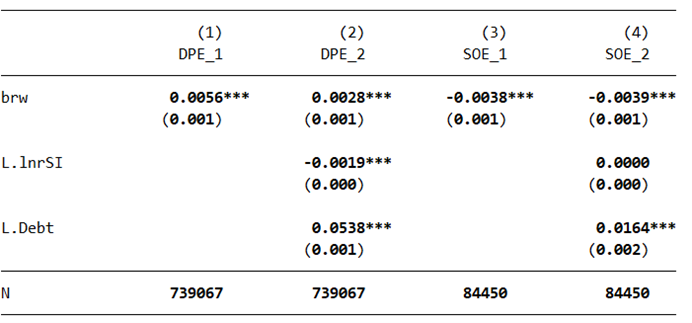
\includegraphics[width=0.9\textwidth]{latex/2023.10/Picture/IEoL_SOE_DPE.png}
         \caption{Impact of US shock on borrowing cost: SOE vs DPE}
         \label{fig:IEoL_SOE_DPE}
\end{figure}

(2) Price response: SOE vs DPE \\
Note: the dependent variable is dlnprice YoY. The prices of SOE are unaffected (see Figure \ref{fig:Price_brw_DPE_SOE}).

\begin{figure}
     \centering
         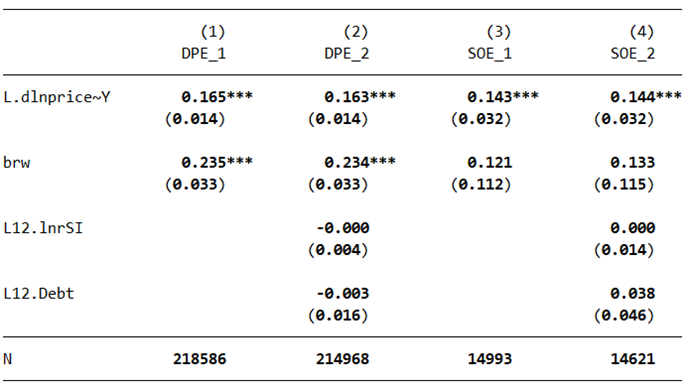
\includegraphics[width=0.9\textwidth]{latex/2023.10/Picture/Price_brw_DPE_SOE.png}
         \caption{Impact of US shock on export price: SOE vs DPE}
         \label{fig:Price_brw_DPE_SOE}
\end{figure}


\textbf{Further check 2: exposure heterogeneity to US shock across industries}

Some industries are more exposed to international financial market, such as the commodities prices, which has very mature global financial market. From this picture, we can see that 25(oil), 26/28(chemistry), 32/33(metal) have much bigger responses compared with other industries (see Figure \ref{fig:Industry}).

\begin{figure}
     \centering
         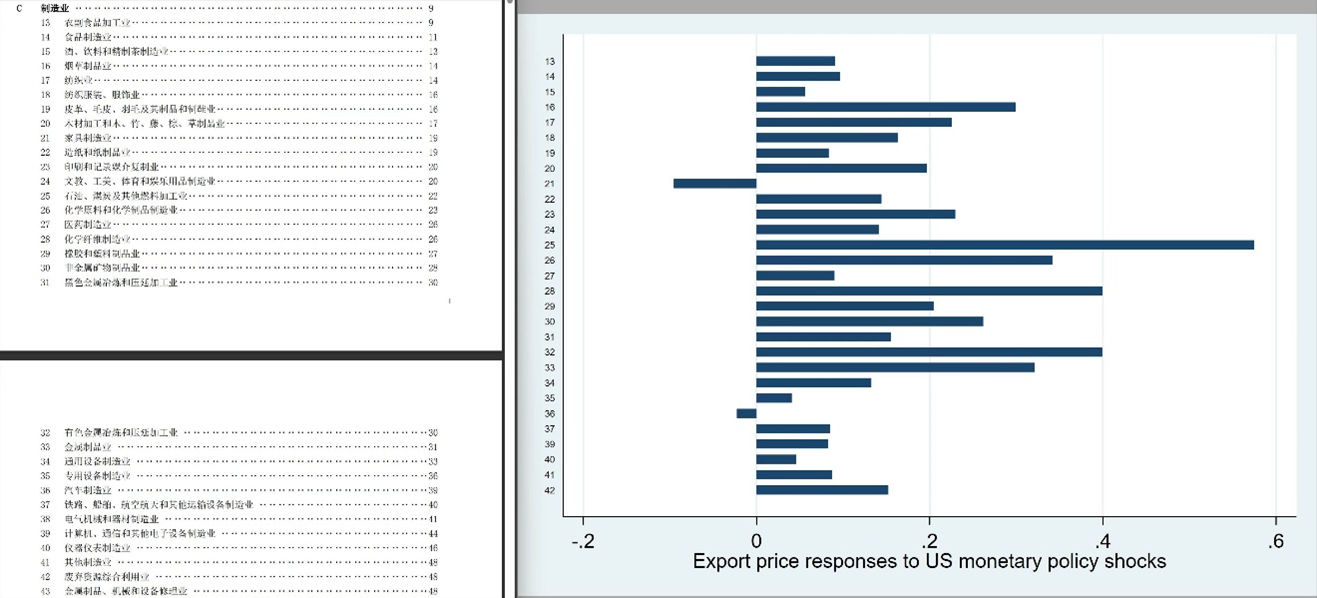
\includegraphics[width=0.9\textwidth]{latex/2023.10/Picture/Industry.png}
         \caption{Impact of US shock on export price across industries}
         \label{fig:Industry}
\end{figure}


\textbf{Further check 3: exposure heterogeneity to US shock across regimes: Fixed VS floating}

“\textit{A large body of this literature has shown that in the post-Bretton Woods period interest rates are more closely linked in countries that peg and in countries with open capital markets compared with countries that do not peg or impose capital restrictions. (See e.g., Klein and Shambaugh (2010).})” -- Dedola, Luca, Giulia Rivolta, and Livio Stracca. "If the Fed sneezes, who catches a cold?." Journal of International Economics 108 (2017): S23-S41.


If the global borrowing cost channel and global liquidity channel hold, then under fixed regime Chinese financial conditions are more exposed to US shock, so we expect that the export prices responses should be larger (see Figure \ref{fig:regime}). 

\begin{figure}
     \centering
         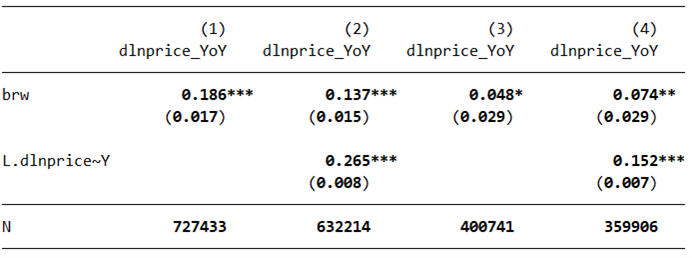
\includegraphics[width=0.9\textwidth]{latex/2023.10/Picture/regime.png}
         \caption{Impact of US shock on export price across regimes}
         \label{fig:regime}
\end{figure}

 
Note: Column (1)(2): fixed regime; Column (3)(4): floating regime


\section{Alternative explanations}

\subsection{Demand side expansion?}

The idea presented is that after a shock, global demand goes up, causing China's export prices to rise. However, if we have a tightening shock, it should lead to reduced demand and lower prices, not an increase. So, the argument about the demand side doesn't make sense. Some people argue that a tightening shock makes Chinese exports more competitive because Chinese products become cheaper compared to similar ones from other countries. They compare this to Giffen goods, where prices go up when people's incomes drop. But this doesn't seem likely because most product prices increase after a shock, especially things like oil and metal related goods, which aren't considered as Giffen goods.

\subsection{Import price increase?}

This story is that China’s export price increases is because the import price increases. To rule out it, we do two tasks:

i. Using the annually firm-product-country level import price data, we replace export price change with import price change in the benchmark level regression and find that results are insignificant

(Update)

ii. Using the annually firm-product-country level export price data, we include brw*import intensity or brw*I(import intensity>pct75). If this story holds, prices should increase more with higher import intensity. But the results are insignificant.

(Update)

\subsection{Exchange rate depreciation induced price increase?}

This story is that export price denominated in RMB increase is just because RMB depreciates against other currencies, so to keep purchasing power of export income unchanged, the firms should increase price. This explanation can be refuted based on two reasons:

i. Our results are also significant before 2005m7, when China’s exchange rate is almost fixed to US dollar, which means that positive brw shock should appreciate RMB against other currencies


ii. Using the annually firm-product-country level export price data, we have controlled the bilateral real exchange rate, and results are robust.

(update)


\section{Model}

\subsection{Baseline model}
Following \cite{melitz2003impact}, \cite{manova2013credit} and \cite{fan2015credit}, here we construct a partial equilibrium micro-founded model to rationalize why firms increase export prices in response to a US monetary contraction and capture how this is related to borrowing cost increase and liquidity constrain. The big picture is that a positive US shock will induce the increase of borrowing rate and thus the marginal cost, and finally the export price. What’s more, liquidity condition is an augmenter of this transmission: the firm will increase more when liquidity is worse.

\subsubsection{Model setting}

\begin{enumerate}
    \item We abstract household part and assume The demand is exogenous and it is a decreasing function of US monetary shock, like IS curve.
    \item Borrowing cost is a function of US monetary shock and the firms take it as exogenous
    \item Constant mark-up\footnote{This is consistent with our empirical result.}
    \item Price is flexible \footnote{We observe that, at the firm level, the export price respond to US shock contemporaneously}
    \item Firm production is a function of labor, capital and inventory (see \cite{corugedo2011understanding})
    \item Firms need to pay the principal and interest of loan by cash;
    \item Firms need to pay the inventory fees and wage by loan\footnote{The working capital constrain is common and realistic for exporting firms. “The notion that exporters depend more on external financing than domestic producers because of additional costs related to trade, greater transaction risks, and higher working capital needs due to longer shipping times.” -- \cite{manova2013credit}};
\end{enumerate}


\subsubsection{Expected outcome}

Our results is expected to be consistent with the "efficiency sorting" discussed in \cite{fan2015credit} (see Figure \ref{fig: FLL_model}) \footnote{Monetary policy is a temporal shock, firms are less likely to adjust the quality. It is hard to imagine, the Fed increase 10bp one-year treasury rate will induce a toy firm to produce low-quality toy cars. So, here we can model in the way of “efficiency sorting”.}. Below is their prediction:



\begin{figure}
     \centering
         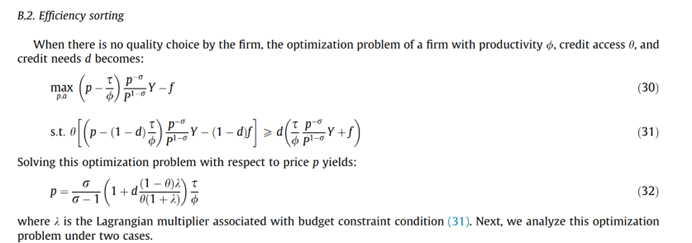
\includegraphics[width=0.9\textwidth]{latex/2023.10/Picture/FLL_model.png}
         \caption{\cite{fan2015credit} model}
         \label{fig: FLL_model}
\end{figure}
 


"\textit{Under quality sorting, tighter credit constraints (i.e., a higher d or a lower h) lower the optimal product quality chosen by a firm and thus reduce the optimal price. In this case, prices increase with productivity, ceteris paribus. However, when there is no quality choice (i.e., under efficiency sorting), given firm productivity, tighter credit constraints (i.e., a higher d or a lower theta) increase the optimal price set by a firm. In this efficiency sorting case, export prices decrease with productivity, ceteris paribus.}" -- \cite{fan2015credit}
 
In our model, Cash ratio is like “1/d”, which means the lower the cash ratio, the more credit is needed. Borrowing cost is like “1/$\theta$”, which means the lower the cost, the easier credit is accessed. It can be proved that tightening monetary shock will worsen firm’s credit conditions. So, “1/d” and  “1/$\theta$” is a function of brw shock. Specifically, brw will decrease cash ratio (this can be achieved through two ways: 1. Positive brw shrink the demand thus decreasing the sales income; 2. Positive shock tightening the credit provision either from banks or trade partners), which causes firms need more credit; also, brw will increase borrowing cost, which makes external credit less accessible. The firm maximization problem is like \cite{corugedo2011understanding} (see Figure \ref{fig: Corugedo_model}), by which we can derive that marginal cost are positively correlated with borrowing cost. Similarly, we can imagine that in the setting of \cite{manova2013credit}, $c_{js}$ is an increasing function of US shock (see Figure \ref{fig: Manova_model}). 


\begin{figure}
     \centering
         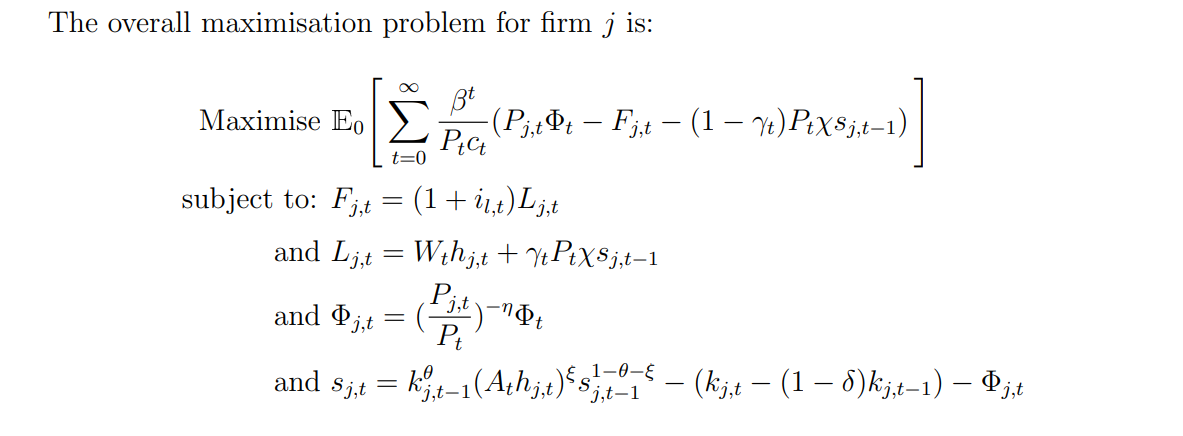
\includegraphics[width=0.9\textwidth]{latex/2023.10/Picture/Corugedo_model.png}
         \caption{\cite{corugedo2011understanding} model}
         \label{fig: Corugedo_model}
\end{figure}


\begin{figure}
     \centering
         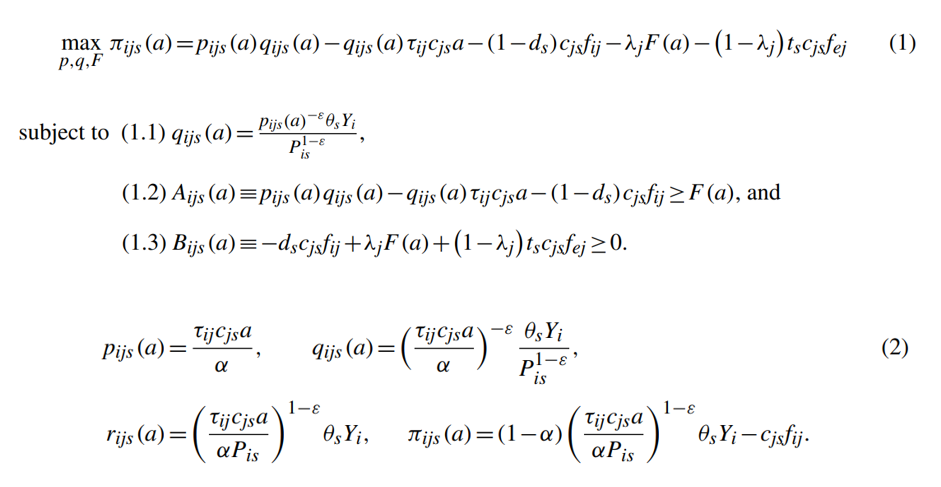
\includegraphics[width=0.9\textwidth]{latex/2023.10/Picture/Manova_model.png}
         \caption{\cite{manova2013credit} model}
         \label{fig: Manova_model}
\end{figure}

The analysis above may be summarized by two propositions:

\textbf{proposition 1} \\
A contractionary US shock will increase borrowing cost, which makes external credit less accessible; and decrease cash ratio, which aggravates firm's credit need

\textbf{proposition 2} \\
Firms will increase export prices in response to a tightening shock and this impact is bigger under higher borrowing cost and lower cash ratio


Following \cite{corugedo2011understanding}, we can also capture trade credit in the model.

Through exogenous parameters setting, we can even write the price as a function of country/sector specific characteristic, so that our model explain cross-country, cross-industry differences.


\subsection{Extension} 

Later, we can relax our assumptions through three lines: (1) endogenize the behavior of banks, or even households; (2) allow mark-up to be variable; (3) assume sticky price, like Calvo type; (4) consider dynamic optimization
; (5) model firm entry and exit











\section{Other issues}

\subsection{About year fixed effect}
Our benchmark level regression should not add year fixed effect. There are several reasons: (i) add year effect will absorb the variation of brw. We only have 7-years monthly data, which is a big loss of variation; (ii) control year effect is to alleviate the concern of omitted variable, which can affect brw and price simultaneously. However, our brw is very exogenous and can’t be affected by other variables; (iii) add year effect has very few benefits because it can only control the annually varying factors but keep silent on other quarterly and monthly level changes; (iv) in the monetary policy shock literature, people don’t control time fixed effect. Chari (2021, RFS) reg monthly capital flow on mps, without control year fixed effect. Lin (2018, JDE) reg annual trade value on mps, doesn’t control decade fixed effect; (v) control year fixed effect, will make the firm-product level regression insignificant, will make firm level regression insignificant in both fixed and floating regime, will make NS shock has a positive effect on dlnprice but negative impact on f.dlnprice. So, to guarantee the consistency of results, I suggest not to control it in our benchmark regression.

\subsection{About cluster level}
Our benchmark now is cluster on firm level. Sometimes this will make some other results also significant, which is difficult to explain. 

\subsection{Why do firms increase prices more under tighter constraints?}

Our measure of FPC doesn’t change across time, so it can’t tell us how firms’ FPC change in response to brw shock. The data reveals that tighter-constrained firms usually have higher prices, which is consistent with Fan, Lai, and Li (2015) (see Figure \ref{fig: FPC_price}). But this doesn’t mean that when there is a contractional brw shock, firms with tighter constrains increase prices more because we don’t how the FPC changes.

\begin{figure}
     \centering
         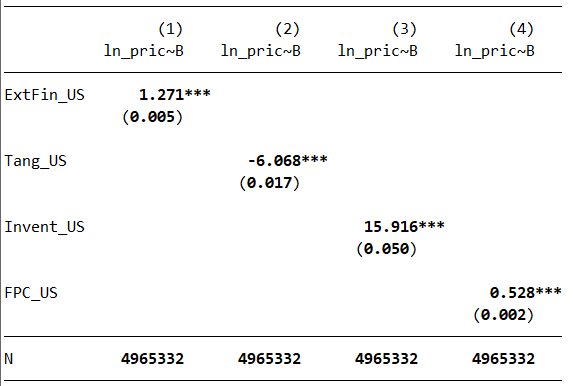
\includegraphics[width=0.9\textwidth]{latex/2023.10/Picture/FPC_price.png}
         \caption{the impact of FPC on price}
         \label{fig: FPC_price}
\end{figure}

The impact of brw*FPC on borrowing cost and cash ratio is insignificant (see Figure \ref{fig: IEOL_Cash_FPC}).

\begin{figure}
     \centering
         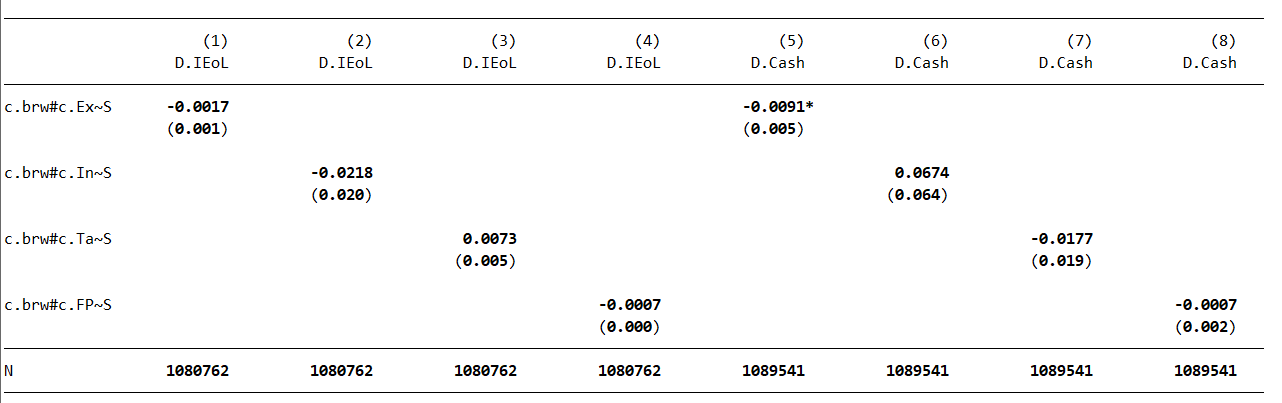
\includegraphics[width=0.9\textwidth]{latex/2023.10/Picture/IEOL_Cash_FPC.png}
         \caption{The imapact of brw on borrowing cost and cash ratio conditional on FPC}
         \label{fig: IEOL_Cash_FPC}
\end{figure}

\subsection{Better to investigate the shocks from all main central banks}

To make our research more general, we'd better examine shocks emanating from all major central banks: the US, Europe, Japan, UK. But there is a question that in our firm-level regression, Japan's shock has a positive effect on export prices if we only cluster on the firm level, which is hard to explain. But this result is not robust, if we cluster on both firm and year-month, this effect will be statistically weak. However, the current regression may not be reasonable, because we don't control exchange rate change. Also, I didn't check the impact in the monthly firm-product-country level regression. I remember in the annual firm-product-country regression, this is insignificant. We need to check this again. Also, we need to check how country X shock affects the export prices to country X, especially to verify the demand shrink effect. Additionally, we should put all the shocks in one equation and see what happens. If we can solve this properly, our paper can go to a better place.

\subsection{Better to explain the difference across country and sectors}

Similarly, to make our research more general, we'd better offer explanations on the differences across countries and sectors. Especially, why the prices of US export doesn't respond. In our current model framework, price is a function of brw and some other exogenous country-sector-specific parameters. The impact of brw is determined by these parameters. As for why the prices of US are insignificant, maybe the demand side and supply side effects are offset because US shock may have a bigger effect on domestic demand and the demand of US-peg countries than other countries. We may still need to regress price change on the interaction term of shock and country/sector-specific characteristics (for country factors: such as gravity controls, financial market development, and financial openness, etc. for sector/product factors: homogeneous or differentiated goods, etc.) to verify which factor drives the differences. 
If we can solve this properly, our paper can go to a better place.

\subsection{The impact between 2008-2015}
Our primary analysis is grounded in the data from 2000 to 2007. Naturally, questions may arise regarding the impact between 2008 and 2015. In our yearly firm-product-country level regression, this period appears statistically insignificant. We have two plausible explanations: Firstly, owing to the zero lower bound, the influence of US monetary policy shocks on global interest rates, particularly short-term rates, has considerably waned. Secondly, noteworthy alterations in China's exchange rate regime, transitioning from a Dollar-targeting approach to a basket-targeting approach, may serve as a mitigating factor in buffering international monetary shocks.

\subsection{Quantity and total value responses}
We can't circumvent this question. Need to add the results.

\subsection{How to model liquidity effect}
Now, how to model the liquidity effect is not quite clear. Still need to read more papers.


\newpage
\bibliography{my.bib}

\end{document}